% TikZ 다이어그램 - 학술 논문 스타일
% 색상 팔레트 정의
\definecolor{primaryblue}{RGB}{31,119,180}
\definecolor{secondaryorange}{RGB}{255,127,14}
\definecolor{accentgreen}{RGB}{44,160,44}
\definecolor{accentpurple}{RGB}{148,103,189}
\definecolor{neutralgray}{RGB}{127,127,127}
\definecolor{lightgray}{RGB}{200,200,200}
\definecolor{hallred}{RGB}{214,39,40}
\definecolor{normgreen}{RGB}{44,160,44}

%=============================================================================
% Figure 1: SE-Gated Cascade 개념도 (깔끔한 플로우차트)
%=============================================================================
\newcommand{\cascadediagram}{
\begin{tikzpicture}[
    node distance=1.5cm,
    >={Stealth[length=2.5mm]},
    box/.style={
        rectangle, draw=black!70, line width=0.8pt,
        rounded corners=2pt, minimum width=3cm, minimum height=0.9cm,
        align=center, font=\small
    },
    inputbox/.style={box, fill=lightgray!30},
    processbox/.style={box, fill=primaryblue!15},
    energybox/.style={box, fill=secondaryorange!20},
    outputbox/.style={box, fill=accentgreen!20},
    decision/.style={
        diamond, draw=black!70, line width=0.8pt,
        aspect=2.5, minimum width=2cm, align=center, font=\small,
        fill=accentpurple!15
    },
    arrow/.style={->, line width=0.8pt, black!70},
    label/.style={font=\scriptsize, text=black!60}
]

% 상단: 입력 → 샘플링 → 클러스터링 (가로)
\node[inputbox] (input) {Input: 질문 $q$};
\node[processbox, right=2cm of input] (sample) {LLM 샘플링 ($K$=5)};
\node[processbox, right=2cm of sample] (cluster) {NLI 클러스터링};

% 중단: 메트릭 계산 (병렬)
\node[processbox, below left=1.5cm and 0.3cm of cluster] (se) {SE 계산};
\node[energybox, below right=1.5cm and 0.3cm of cluster] (energy) {Energy 계산};

% 하단: 분기 및 출력
\node[decision, below=2.5cm of cluster] (gate) {$|C|=1$?};
\node[outputbox, below=1.8cm of gate] (output) {환각 점수};

% 화살표
\draw[arrow] (input) -- (sample);
\draw[arrow] (sample) -- (cluster);
\draw[arrow] (cluster) -- (se);
\draw[arrow] (cluster) -- (energy);
\draw[arrow] (se) -- (gate);
\draw[arrow] (energy) -- (gate);
\draw[arrow] (gate) -- node[right, label] {Energy (Yes) / SE (No)} (output);

% 클러스터 수 표시
\node[font=\scriptsize, text=black!50, right=0.1cm of cluster] {$\rightarrow |C|$};

\end{tikzpicture}
}

%=============================================================================
% Figure 2: Zero-SE 현상 요약 (3-panel)
%=============================================================================
\newcommand{\zerosefigure}{
\begin{tikzpicture}
% Panel A: 도넛 차트
\begin{scope}[local bounding box=panelA]
    \def\innerrad{0.7}
    \def\outerrad{1.4}
    % Non-Zero-SE (81%)
    \fill[primaryblue!60] (90:\outerrad) arc (90:-201.6:\outerrad) -- (-201.6:\innerrad) arc (-201.6:90:\innerrad) -- cycle;
    % Zero-SE (19%)
    \fill[hallred!70] (90:\outerrad) arc (90:90-68.4:\outerrad) -- (21.6:\innerrad) arc (21.6:90:\innerrad) -- cycle;
    
    % 중앙 텍스트
    \node[font=\small\bfseries] at (0,0) {n=200};
    
    % 범례
    \node[font=\scriptsize, anchor=west] at (1.8, 0.4) {\textcolor{hallred!70}{$\blacksquare$} Zero-SE (19\%)};
    \node[font=\scriptsize, anchor=west] at (1.8, -0.1) {\textcolor{primaryblue!60}{$\blacksquare$} Non-Zero (81\%)};
    
    \node[font=\small\bfseries, anchor=north] at (0, -1.7) {(a) Zero-SE 비율};
\end{scope}

% Panel B: 환각/정상 구성
\begin{scope}[xshift=6cm]
    \begin{axis}[
        ybar,
        width=4.5cm, height=4.5cm,
        ymin=0, ymax=35,
        xtick={1,2},
        xticklabels={환각, 정상},
        ylabel style={font=\scriptsize},
        xlabel style={font=\scriptsize},
        tick label style={font=\scriptsize},
        bar width=12pt,
        nodes near coords,
        nodes near coords style={font=\scriptsize},
        axis lines=left,
        enlarge x limits=0.5,
        title={\small\bfseries (b) Zero-SE 구성},
        title style={at={(0.5,1.05)}},
    ]
    \addplot[fill=hallred!70, draw=hallred!90] coordinates {(1,28)};
    \addplot[fill=normgreen!60, draw=normgreen!80] coordinates {(2,10)};
    \end{axis}
    \node[font=\tiny, text=black!60] at (1.8, 3.8) {환각률: 73.7\%};
\end{scope}

% Panel C: Energy AUROC
\begin{scope}[xshift=10.5cm]
    \begin{axis}[
        ybar,
        width=4cm, height=4.5cm,
        ymin=0, ymax=1,
        xtick={1},
        xticklabels={Energy},
        ylabel={AUROC},
        ylabel style={font=\scriptsize},
        tick label style={font=\scriptsize},
        bar width=20pt,
        nodes near coords,
        nodes near coords style={font=\scriptsize},
        axis lines=left,
        enlarge x limits=1,
        title={\small\bfseries (c) Zero-SE 탐지},
        title style={at={(0.5,1.05)}},
        extra y ticks={0.5},
        extra y tick style={grid=major, grid style={dashed, lightgray}},
        extra y tick labels={},
    ]
    \addplot[fill=secondaryorange!70, draw=secondaryorange!90] coordinates {(1,0.736)};
    \end{axis}
    \node[font=\tiny, text=black!50] at (1.2, 2) {random=0.5};
\end{scope}
\end{tikzpicture}
}

%=============================================================================
% Figure 3: SE vs Energy Crossover (Grouped Bar)
%=============================================================================
\newcommand{\crossoverfigure}{
\begin{tikzpicture}
\begin{axis}[
    ybar,
    width=11cm, height=6.5cm,
    bar width=14pt,
    ylabel={AUROC},
    ylabel style={font=\small},
    ymin=0, ymax=0.9,
    xtick={1,2,3},
    xticklabels={Zero-SE\\{\tiny $|C|=1$}, Medium\\{\tiny $0.5<\text{SE}\leq1$}, High\\{\tiny $\text{SE}>1$}},
    xticklabel style={align=center, font=\small},
    tick label style={font=\small},
    legend style={
        at={(0.98,0.98)}, anchor=north east, 
        font=\small, 
        draw=none, fill=white, fill opacity=0.8,
        legend columns=1
    },
    nodes near coords,
    nodes near coords style={font=\scriptsize, /pgf/number format/.cd, fixed, precision=2},
    axis lines=left,
    enlarge x limits=0.25,
    extra y ticks={0.5},
    extra y tick style={grid=major, grid style={dashed, lightgray, line width=0.5pt}},
    extra y tick labels={},
    ymajorgrids=false,
]
\addplot[fill=primaryblue!70, draw=primaryblue] coordinates {(1,0.001) (2,0.61) (3,0.66)};
\addplot[fill=secondaryorange!70, draw=secondaryorange] coordinates {(1,0.74) (2,0.52) (3,0.42)};
\legend{SE, Energy}
\end{axis}

% 주석
\node[font=\scriptsize, text=secondaryorange!80!black, anchor=west] at (1.2, 5.2) {$\leftarrow$ Energy 우세};
\node[font=\scriptsize, text=primaryblue!80!black, anchor=east] at (9.5, 5.2) {SE 우세 $\rightarrow$};
\draw[->, line width=0.6pt, secondaryorange!70] (2.5, 5.0) -- (1.5, 4.5);
\draw[->, line width=0.6pt, primaryblue!70] (8, 5.0) -- (9, 4.5);

\end{tikzpicture}
}

%=============================================================================
% Figure 4: 상보성 분석 (Stacked/Grouped)
%=============================================================================
\newcommand{\complementarityfigure}{
\begin{tikzpicture}
\begin{axis}[
    ybar,
    width=10cm, height=6cm,
    bar width=22pt,
    ylabel={환각 샘플 수 (n=164)},
    ylabel style={font=\small},
    ymin=0, ymax=130,
    xtick={1,2,3,4},
    xticklabels={SE만\\탐지, Energy만\\탐지, 둘 다\\탐지, 미탐지},
    xticklabel style={align=center, font=\small},
    tick label style={font=\small},
    nodes near coords,
    nodes near coords style={font=\scriptsize},
    axis lines=left,
    enlarge x limits=0.2,
]
\addplot[fill=primaryblue!70, draw=primaryblue] coordinates {(1,22) (2,0) (3,0) (4,0)};
\addplot[fill=secondaryorange!70, draw=secondaryorange] coordinates {(1,0) (2,22) (3,0) (4,0)};
\addplot[fill=accentpurple!60, draw=accentpurple] coordinates {(1,0) (2,0) (3,12) (4,0)};
\addplot[fill=neutralgray!50, draw=neutralgray] coordinates {(1,0) (2,0) (3,0) (4,108)};
\end{axis}

% 비율 레이블
\node[font=\tiny, text=black!60] at (1.5, 2.2) {13.4\%};
\node[font=\tiny, text=black!60] at (3.6, 2.2) {13.4\%};
\node[font=\tiny, text=black!60] at (5.7, 1.5) {7.3\%};
\node[font=\tiny, text=black!60] at (7.8, 4.8) {65.9\%};

% 합집합 강조 박스
\draw[rounded corners=3pt, fill=accentgreen!10, draw=accentgreen!50, line width=0.8pt] 
    (0.3, 5.3) rectangle (5, 6.2);
\node[font=\small, text=accentgreen!80!black] at (2.65, 5.75) {합집합 탐지율: \textbf{34.1\%}};

\end{tikzpicture}
}

%=============================================================================
% Figure 5: 전체 성능 비교 (Simple Bar)
%=============================================================================
\newcommand{\overallfigure}{
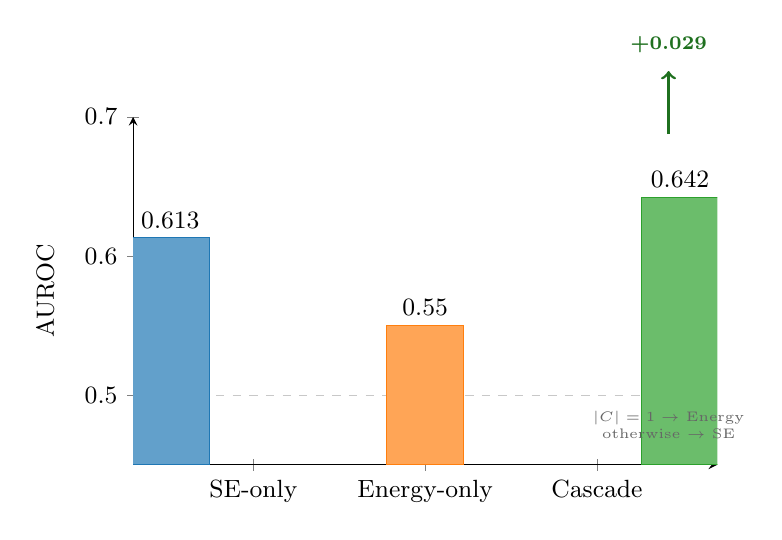
\begin{tikzpicture}
\begin{axis}[
    ybar,
    width=9cm, height=6cm,
    bar width=28pt,
    ylabel={AUROC},
    ylabel style={font=\small},
    ymin=0.45, ymax=0.70,
    xtick={1,2,3},
    xticklabels={SE-only, Energy-only, Cascade},
    xticklabel style={font=\small},
    tick label style={font=\small},
    nodes near coords,
    nodes near coords style={font=\small, /pgf/number format/.cd, fixed, precision=3},
    axis lines=left,
    enlarge x limits=0.35,
    extra y ticks={0.5},
    extra y tick style={grid=major, grid style={dashed, lightgray}},
    extra y tick labels={},
]
\addplot[fill=primaryblue!70, draw=primaryblue] coordinates {(1,0.613)};
\addplot[fill=secondaryorange!70, draw=secondaryorange] coordinates {(2,0.550)};
\addplot[fill=accentgreen!70, draw=accentgreen] coordinates {(3,0.642)};
\end{axis}

% 개선 화살표
\draw[->, line width=1pt, accentgreen!70!black] (6.8, 4.2) -- (6.8, 5.0);
\node[font=\scriptsize, text=accentgreen!70!black, anchor=south] at (6.8, 5.1) {\textbf{+0.029}};

% Cascade 설명
\node[font=\tiny, text=black!60, align=center, anchor=north] at (6.8, 0.8) {$|C|=1 \rightarrow$ Energy\\otherwise $\rightarrow$ SE};

\end{tikzpicture}
}
